% Drawing 154/03-11 -- folder 154, batch 03, archive page 41 (PDF page 42).
% Transcription: figure au bas de la colonne de gauche : un disque au bord vert (clair à gauche, foncé à droite), traversé de cordes orange ; une corde verticale en pointillé vert et bleu joint en haut les points marqués $y$, $x$ à ceux marqués $y'$, $x'$ en bas ; la moitié gauche du disque est hachurée au crayon, la moitié droite striée de traits noirs horizontaux ; $D$ est marqué près de la corde, $a$ à droite sur le bord
% Kind: disk cut by a dotted chord, hatched halves. Method 2 (schematic redraw from the facsimile). Status: partial.
% Notes: Rim light green on the left of the dotted chord, dark green on its right; the dark green dotted chord, slightly bowed, with five black points (one near the top, two close together at the middle, one lower down, one at its foot where two strands meet). Orange strands: on the left of the chord two strands from the top rim down to the black point at the foot; a strand from the upper right rim through the upper black point, joining the inner of those two lower down; one strand right of the chord from top to bottom; three strands from the left rim to the two middle black points, and from there a fan of three strands to the right rim; a long strand from the upper left rim down across the left half and over to the lower right rim; a short strand from the bottom rim up to the vertical strands. Pencil hatching on the left half; thirteen horizontal black strokes on the right half. Labels y, x above, y', x' below, D four times (the two upper left ones carry an index that is not legible and is left out), a on the right. Redrawn 2026-11-12 (issue 128). 2026-11-14, Claude Opus 5.5, second pass (issue 147): redrawn strand by strand from the 400 dpi colour crop, every stroke through points measured on the colour mask of its ink (orange, light and dark green) or on its darkness along rows and columns of a unit grid; the rim, the chord (it was straight and 1 to 2 units off), the eleven orange strands (five of them were 2 to 5 units off), the black points, the thirteen black strokes (eight were drawn, some 3 to 7 units too long) and the labels. Overlay: every orange strand, the rim, the chord and the black strokes lie on their ink (mean distance under 0.5 unit). Still differs: the pencil hatching of the left half is drawn as a pattern of vertical lines filling the half-disk, where the page has dense wavy vertical pencil strokes, partly under the orange strands, leaving a margin along the rim at the upper left; they are not drawn one by one. Not compiled (no TeX in the session). Not checked by a reader.
% Coordinates: 1 unit = 1 mm = 1/100 of the crop width (bbox in page fractions: [0.135, 0.325, 0.275, 0.445]).
% Redrawn by Claude (claude-fable-5-2), issue #128, 2026-11-12; not checked by a human; not compiled (no TeX in the session).
% Redrawn stroke by stroke by Claude (claude-opus-5-5) 2026-11-14 (issue #147, second pass): overlaid on the 400 dpi colour facsimile on a unit grid; not compiled (no TeX in the session). Not checked by a human. Status: partial.
% Rights: reproduces part of the work -- behind RENDER_TRANSCRIPTS, never published by itself.
\documentclass[tikz,border=3pt]{standalone}
\usepackage{amsmath,amssymb}
\usetikzlibrary{patterns,arrows.meta}
\tikzset{Or/.style={orange!90!black}, Lg/.style={green!60!black!70}, Dg/.style={green!45!black}, pencil/.style={black!45}, struck/.style={black!35}, mpt/.style={circle,draw,inner sep=1.3pt}, pt/.style={circle,fill,inner sep=0.9pt}, opt/.style={circle,draw,fill=white,inner sep=1.1pt}}
\begin{document}
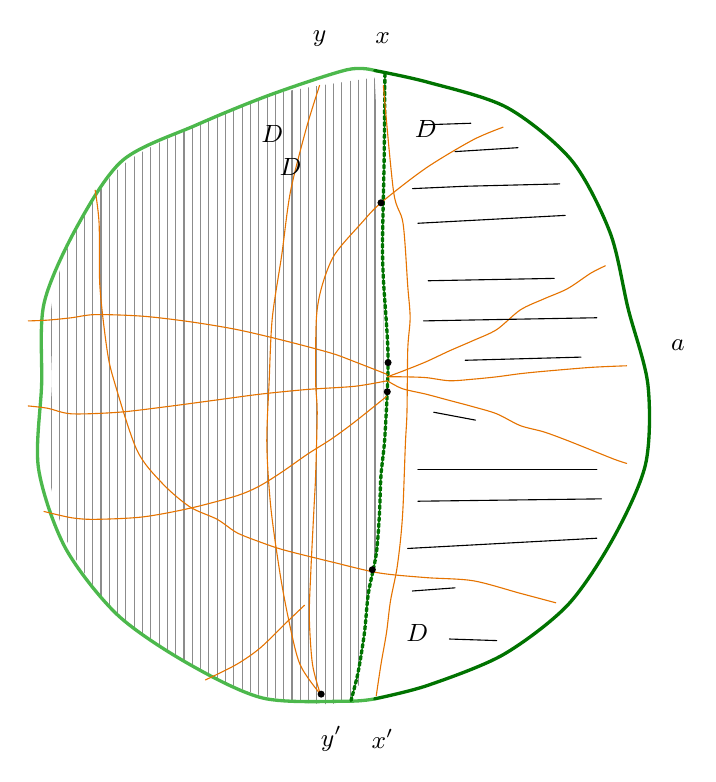
\begin{tikzpicture}[x=1mm,y=1mm,line cap=round,line join=round,font=\scriptsize]
\fill[pattern=vertical lines,pattern color=black!45] plot[smooth, tension=0.5] coordinates {(58.5,-19.5) (45.2,-21.7) (35.9,-25.5) (26.5,-30.6) (20.6,-38.6) (17.5,-48.2) (17.5,-58.5) (17,-69.1) (19.8,-79.2) (25.8,-87.7) (34.6,-93.8) (44.3,-98) (55.5,-98.4) (57.5,-88) (58.8,-78) (59.6,-60) (59.5,-40)} -- cycle;
\draw[Lg,very thick] plot[smooth, tension=0.5] coordinates {(58.5,-18.6) (55,-18.5) (45.2,-21.7) (35.9,-25.5) (26.5,-30) (20.6,-38.6) (16.5,-48.2) (16.2,-58.5) (15.8,-69.1) (19.2,-79.2) (25.8,-87.7) (34.6,-93.8) (44.3,-98.3) (55,-98.7) (58.5,-98.4)};
\draw[Dg,very thick] plot[smooth, tension=0.5] coordinates {(58.5,-98.4) (65.2,-96.7) (74.8,-92.8) (83,-86.5) (88.8,-78) (92.9,-68.6) (93.2,-58.5) (90.7,-48.9) (88.4,-39.2) (83.5,-30) (75.3,-23.3) (65.3,-20.1) (58.5,-18.6)};
\draw[Dg,densely dotted,very thick] plot[smooth, tension=0.5] coordinates {(59.8,-19) (59.7,-30) (59.5,-40) (59.6,-45) (60.2,-55) (59.8,-65) (59.3,-70) (59.1,-75) (58.7,-80) (57.7,-85) (57.2,-90) (56.4,-95) (55.5,-98.6)};
\draw[Or] plot[smooth, tension=0.5] coordinates {(51.5,-20.5) (49.8,-26) (47.8,-34) (46.7,-42) (45.5,-50) (45.1,-58) (44.8,-66) (45.3,-74) (46.4,-82) (47.5,-88) (49,-94) (51.6,-97.8)};
\draw[Or] plot[smooth, tension=0.5] coordinates {(74.8,-25.8) (71,-27.4) (65,-31) (59.3,-35.4) (56.8,-38) (53.4,-42) (51.8,-46) (51.1,-50) (51,-58) (51.2,-62) (51,-70) (50.8,-74) (50.4,-82) (50.2,-88) (50.6,-94) (51.6,-97.8)};
\draw[Or] plot[smooth, tension=0.5] coordinates {(59.6,-20.5) (60.9,-34) (62.1,-38) (62.7,-46) (63,-50) (62.7,-54) (62.6,-62) (62.4,-66) (62.1,-74) (61.8,-78) (61.3,-82) (60.5,-86) (60,-90) (59.3,-94) (58.7,-98)};
\draw[Or] plot[smooth, tension=0.5] coordinates {(14.5,-50.4) (17,-50.3) (20,-50) (23,-49.6) (29,-49.8) (35,-50.5) (41,-51.5) (47,-52.9) (53,-54.5) (56,-55.6) (60.1,-57.2)};
\draw[Or] plot[smooth, tension=0.5] coordinates {(14.5,-61.2) (17,-61.5) (20,-62.2) (26,-62) (32,-61.3) (38,-60.5) (44,-59.7) (50,-59.1) (56,-58.7) (60.1,-58)};
\draw[Or] plot[smooth, tension=0.5] coordinates {(16.5,-74.6) (20,-75.4) (23,-75.6) (29,-75.3) (35,-74.2) (41,-72.6) (44,-71.3) (47,-69.4) (50,-67.3) (53,-65.4) (56,-63.2) (60,-60)};
\draw[Or] plot[smooth, tension=0.5] coordinates {(23,-33.8) (23.5,-38) (23.6,-46) (24.5,-54) (25.4,-58) (28.3,-66.8) (31.5,-71) (35,-74) (38.5,-75.6) (41,-77.3) (44,-78.5) (47,-79.5) (53,-81) (59,-82.4) (65,-83) (71,-83.4) (77,-85) (81.5,-86.2)};
\draw[Or] plot[smooth, tension=0.5] coordinates {(37,-96) (41,-94) (44,-91.9) (47.5,-88.5) (49.6,-86.5)};
\draw[Or] plot[smooth, tension=0.5] coordinates {(60.1,-57.5) (62,-56.8) (65,-55.6) (68,-54.2) (71,-52.9) (74,-51.5) (77,-49) (80,-47.6) (83,-46.3) (86,-44.3) (87.8,-43.4)};
\draw[Or] plot[smooth, tension=0.5] coordinates {(60.1,-57.5) (62,-57.5) (65,-57.6) (68,-58) (71,-57.8) (74,-57.5) (77,-57.1) (80,-56.8) (86,-56.3) (90.5,-56.1)};
\draw[Or] plot[smooth, tension=0.5] coordinates {(60.1,-58) (62,-59) (65,-59.7) (68,-60.5) (71,-61.3) (74,-62.2) (77,-63.7) (80,-64.5) (83,-65.6) (86,-66.8) (89,-68) (90.5,-68.5)};
\draw (64.7,-25.5) -- (70.7,-25.3);
\draw (68.7,-28.9) -- (76.7,-28.4);
\draw (63.3,-33.6) -- (70,-33.3) -- (82,-33);
\draw (64,-38) -- (82.7,-37);
\draw (65.3,-45.3) -- (81.3,-45);
\draw (64.7,-50.4) -- (70,-50.3) -- (86.7,-50);
\draw (70,-55.4) -- (84.7,-55);
\draw (66,-62) -- (71.3,-63);
\draw (64,-69.3) -- (86.7,-69.3);
\draw (64,-73.3) -- (87.3,-73);
\draw (62.7,-79.3) -- (86.7,-78);
\draw (63.3,-84.7) -- (68.7,-84.3);
\draw (68,-90.8) -- (74,-91);
\node[pt] at (59.3,-35.4) {};
\node[pt] at (60.2,-55.7) {};
\node[pt] at (60.1,-59.4) {};
\node[pt] at (58.2,-82) {};
\node[pt] at (51.7,-97.8) {};
\node[inner sep=1pt] at (51.5,-14.5) {\small $y$};
\node[inner sep=1pt] at (59.5,-14.5) {\small $x$};
\node[inner sep=1pt] at (53,-103.5) {\small $y'$};
\node[inner sep=1pt] at (59.5,-103.5) {\small $x'$};
\node[inner sep=1pt] at (45.5,-26.7) {\small $D$};
\node[inner sep=1pt] at (47.8,-30.8) {\small $D$};
\node[inner sep=1pt] at (65,-26) {\small $D$};
\node[inner sep=1pt] at (63.9,-90) {\small $D$};
\node[inner sep=1pt] at (97,-53.5) {\small $a$};
\end{tikzpicture}
\end{document}
